\documentclass[justified,notitlepage]{tufte-book}   	
% use "amsart" instead of "article" for AMSLaTeX format
%\usepackage{geometry}                		% See geometry.pdf to learn the layout options. There are lots.
%\geometry{letterpaper}                   		% ... or a4paper or a5paper or ... 
%\geometry{landscape}                		% Activate for for rotated page geometry
%\usepackage[parfill]{parskip}    		% Activate to begin paragraphs with an empty line rather than an indent
\usepackage{appendix}
\usepackage{graphicx}				% Use pdf, png, jpg, or eps with pdflatex; use eps in DVI mode
\usepackage[plain]{fancyref}								% TeX will automatically convert eps --> pdf in pdflate
\usepackage{amsmath}
\usepackage{mathtools}	
\usepackage{amssymb}
\usepackage{amsthm}

%\newcommand*{\fancyrefthmlabelprefix}{eq}
\newcommand*{\fancyrefthmlabelprefix}{thm}
\frefformat{plain}{\fancyrefthmlabelprefix}{theorem~#1}
\Frefformat{plain}{\fancyrefthmlabelprefix}{Theorem~#1}
\newcommand*{\fancyrefapplabelprefix}{app}
\frefformat{plain}{\fancyrefapplabelprefix}{appendix~#1}
\Frefformat{plain}{\fancyrefapplabelprefix}{Appendix~#1}
\title{Optimal Population Coding of Dynamic Stimuli}
\author{Alex Kunze Susemihl}
%\date{}							% Activate to display a given date or no date

\begin{document}
\maketitle
\setcounter{secnumdepth}{1}
\tableofcontents
\chapter{Introduction}

\newthought{Neuroscience as a whole} is concerned with the function of the nervous system. More precisely, it asks a very simple question: {\em What is the brain doing?}\footnote{ Or alternatively: {\em What is the nervous system doing?}} The simplicity with which humans and animals perform in their environment makes it almost unnatural to ask how their brains enable these behaviors. It is often hard to explain to laymen the complexity involved in preparing even the simplest actions, such as saccades or walking, such is the ease with which these are normally performed. Although one can not realistically expect to answer that question in any general fashion, I will try to touch upon a number of points which shed light on some aspects of the nervous system and provide us with a {\em guiding principle} to understand what the brain is doing and why and possibly how.\par
Neuroscience was born as a branch of biology, and although it is now often thought of as  an interdisciplinary science in itself, its objects of study are still to a large extent biological systems. Theodosius Dobzhansky published an influential essay in 1973, entitled {\em Nothing in biology makes sense except in the light of evolution}\cite{Dobzhansky1973}, which defends exactly that point. Though it has been reviewed and revisited constantly since its proposal, the theory of evolution through natural selection remains the central pillar of biological sciences. As such, neuroscience must also view its objects of study through the lenses of evolution. More specifically, we can then ask ourselves {\em What evolutionary advantage would this brain bring to an individual?} instead of {\em Why is the brain this way?} That being said,  there are caveats in the case of neuroscience. For one, the brain is capable of plasticity and adaptation unthinkable for other organs, and so we can not expect to understand the functionality of the brain in the same way in which the shape of bird beaks can be understood as a function of their preferred fruits and seeds. Furthermore, the brain controls all of the motor and perceptual apparatus, having a multitude of uses and purposes, unlike simpler organs.\par
One particular aspect of the brain which has received increasing attention recently is its ability to deal with uncertainty. In a very productive line of research, a number of experiments have demonstrated that human and animal integrate uncertain information in a near-optimal way. The so-called {\em Bayesian Brain}\cite{Knill2004}, would explicitly represent the distribution over world states and perform inference in a manner consistent with Bayesian inference, obtaining optimal integration of sensory cues from different modalities, for example. It is still a matter of debate how these Bayesian computations would be implemented in the brain. One possibility is that the activity of neurons is sampling from a representation of the distribution of world states\cite{Berkes2011}, which is frequently called the {\em sampling hypothesis}. Another is that the activity of the neurons itself represents the likelihood over world states\cite{Ma2006}, and the population as a whole codes for the distribution, hence the term {\em population coding}.\par

\subsection*{Structure}
\newthought{The main goal of this thesis} is to develop a conceptual framework for studying optimal population coding in a dynamic framework. Furthermore, I would like to establish a link between optimal dynamic encoders and the efficient coding hypothesis, first proposed by Horace Barlow\cite{Barlow1961}. I believe that the inclusion of time into the coding framework raises a number of questions, which have not been addressed in the scientific literature properly. In the remainder of this chapter, I will discuss the efficient coding hypothesis and its more recent developments, and I will touch upon its relationship to Shannon's information theory\cite{Shannon1948}. I will finish by discussing the issue of dynamic population coding, highlighting the issues which I believe are of importance in considering the temporal aspect of coding. I will make the case for a study of optimal filtering of partially observed stimuli as a model of stimulus inference based on spike trains. Following, in \fref{chap:filtering}  I will introduce the general theory of filtering of stochastic stimuli. After that, in \fref{chap:MSE} I will discuss results regarding the Mean-Squared-Error (MSE) of optimal filters of point process data, presenting a number of new analytical results. In \fref{chap:control}, I will generalize the filtering framework to control problems, showing results for optimal control theory of point process-observed processes. In \fref{chap:optimal} I will then provide the connection to neuroscience, by considering the optimal encoding strategy for a population of neurons coding for a stochastic stimulus. I will then finalize by discussing the impact of the work presented and suggesting future research directions.\par

\subsection*{Contribution}
\newthought{The main contribution of this thesis} is in providing a conceptual toolbox to study optimal coding problems in a dynamic environment. I propose that the study of the average performance of an optimal Bayesian filter reconstructing the relevant stimulus provides a good measure of the quality of a dynamic code. Using this framework, I derive analytical results for the fast population code for dense populations of Gaussian neurons proposed by Quentin Huys\cite{Huys2007}. These are to my best knowledge the first results of this kind obtained for temporal coding of dynamic stimuli.

\section{Efficient Coding Hypothesis}

\newthought{The information} associated with a random event is defined as the logarithm of its inverse probability. We can further define the entropy of a distribution over a set of events as the average information conveyed by these events. So if we have a random variable $X$ taking values $x \in \mathcal{A}_X$ and a probability distribution $P : \mathcal{A}_X \to [0,1]$, we will have
$$
H(X)= \sum_x P_X(x) \log\left(\frac{1}{P_X(x)}\right).
$$
The entropy measures how much information is gained from a random observation of $X$ on average, and is usually thought of as a measure of the uncertainty or disorder in the distribution $P_X$. Its unit is usually defined as the {\em bit}, derived from binary digit, when the logarithm is taken in base 2. So, a distribution where we have $P_X(x^*) = 1$ for some $x^*$ and $P_X(x) = 0$ for all other $x\neq x^*$ would have an entropy of $0$, since our measurement gives us an average information of $0$. The outcome $x^*$ is completely non-informative, and all other outcomes, while infinitely informative have a zero probability of happening.\par
It can also easily be seen that in the absence of other constraints, if the set of outcomes $\mathcal{A}_X$ is finite, the entropy is maximized by the uniform distribution over outcomes $x$, which would give us the maximal average information per observation of the variable $X$\footnote{We provide a short demonstration in \fref{app:entropy}}. In information theory, the entropy provides the number of bits it takes, on average, to specify an outcome of the random variable $X$.\par
We can now define the conditional entropy of two random variables $X$ and $Y$ as
$$
H(Y|X) = \sum_x P_X(x) \sum_y P_Y(y|x) \log\left(\frac{1}{P_Y(y|x)}\right),
$$
i.e. the conditional entropy is the average entropy of $Y$ given $X$, averaged over $X$. This gives us the remaining uncertainty in $Y$ after $X$ has been observed averaged over all outcomes of $X$, or alternatively, the number of bits required to code for an outcome of $Y$ given an outcome of $X$, on average. Let us also define the mutual information between $Y$ and $X$ as
$$
I(X;Y) = H(Y) - H(Y|X) = H(X) - H(X|Y) = I(Y;X).
$$
In line with our interpretation of the conditional entropy, this would give us the average reduction of uncertainty in $Y$ given the observation of $X$ or vice-versa. Note that, if we fix the distribution of $X$ (or $Y$), the mutual information is always maximized if the conditional entropy $H(X|Y)$ (or $H(Y|X)$, respectively) is minimized. It is easy to see that if $P_X(x|y)$ ($P_Y(y|x)$) is given by a one-to-one mapping between $X$ and $Y$, the conditional entropy is zero, as no uncertainty is left in $X$ after the observation of $Y$ (no uncertainty in $Y$ is left after the observation of $X$).\par
Shannon regarded a noisy communication channel as a set of two random variables, one representing the codeword to be transmitted ($X$) and another representing the message received ($Y$). The noise in the channel would then be given by the conditional distribution of received messages given the transmitted codewords ($P_Y(y|x)$). The capacity of this channel is then given by
$$
C = \max_{P_X} I(X;Y).
$$
This is the maximum amount of information we can transmit through a noisy channel given by the distribution $P_Y(Y|X)$.
The rate of a given code is given by the number of bits needed to represent $X$ divided by the number of bits needed to represent $Y$, so if to send a one-bit message $x$ we must transmit a three-bit codeword $y$, our code would have a rate of $1/3$.
The noisy-channel coding theorem\cite{mackay2003information} then states
\newtheorem{noisychannel}{Theorem}
\begin{noisychannel}
\label{thm:noisychannel}
For every discrete memoryless channel with capacity $C$, for any $\epsilon>0$, any rate $R<C$, and for large enough $N$, there exists a code of length $N$ and rate $\leq R$ and a decoding algorithm such that the maximal probability of block error is $\epsilon$.
\end{noisychannel}
Before Shannon's work, it was generally believed that to achieve a vanishingly small error one would need a code with vanishingly small rate. The theorem shows, however, that one can achieve any rate below the channel capacity asymptotically.\par
Shannon's work had profound impacts throughout science and technology. Horace Barlow proposed to use the redundancy of a code as a measure of its inefficiency. The redundancy of a code is given by
$$
\mathcal{R} = 1 - \frac{I(X;Y)}{C},
$$
and it quantifies how {\em efficiently} a given code encodes codewords $x$ into messages $y$. Note that in the case of a noiseless channel, this reduces to 
$$
\mathcal{R} = 1 - \frac{H(X)}{C}= 1 - \frac{H(Y)}{C}.
$$
The limit given by \fref{thm:noisychannel} then gives us the perfect redundancy-free channel. The {\em efficient coding hypothesis}, first proposed by Barlow\cite{Barlow1961} states that sensory relays in the nervous system recode the	messages to reduce the redundancy in them. This allows us to relate the distribution of the codewords in nature, given by the stimulus statistics, to the firing statistics of the nervous system.\par
In one popular example, Simon Laughlin related the distribution of contrasts in the natural environment of the blowfly to the tuning function of the large monopolar cells (LMC's) in the blowfly's visual system\cite{Laughlin1981}. These cells respond to the contrast level in a specific area of the visual field.
Since we are considering only one neuron, the analysis is somewhat simplified. Let us also assume that the activity of the neuron $o$ can be restricted between no response and a maximal response $o_{max}$. We can then write the activity of the neuron as a function of the contrast $c$ as $o = g(c)$. We will then have that the redundancy of the firing is given by
$$
\mathcal{R} = \frac{1}{C} \left(C - H(O) \right),
$$
which is maximized when all output levels are equally probable.
The transformation from contrasts to firing rates can be written as a simple change of variables and we have, after setting $P(o) = \alpha$\marginnote{This is a reverse application of the inverse transform method.}
$$
P(o) do = P(c) dc, \textrm{ and therefore } o(c) = \frac{1}{\alpha} \int_{-1}^c P(c') dc',
$$
as is shown in \fref{fig:laughlin}. This can be generalized to a number of cases, and Atick\cite{Atick1992} provided a thorough review of the framework.\par

\begin{marginfigure}
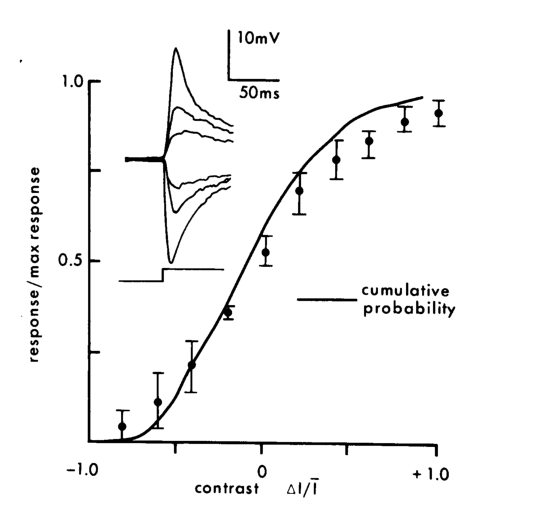
\includegraphics[width=\columnwidth]{figures/laughlin_81.eps}
\label{fig:laughlin}
\caption{The response function of the blowfly LMC closely resembles the cumulative distribution of visual contrasts in its natural environment. Figure taken from Laughlin, S. (1981)}
\end{marginfigure}

This framework can also be generalized to a population of neurons. Writing $O_i$ for the random variable associated with the output activity of each neuron and $O$ for the population activity, we can decompose the redundancy into two terms, yielding
$$
\mathcal{R} = \frac{1}{C} \left(C - \sum_i H(O_i) \right) + \frac{1}{C}\left(\sum_i H(O_i) -H(O)\right).
$$
The first term accounts for redundancy arising from unequal frequency of use of different symbols and the second accounts for redundancy arising from correlations between the activities $O_i$. In the example above we have only had to deal with the left term, since we had only one activity and therefore no correlations between them. A lot of the efficient coding literature, however, has dealt with the second term, and a number of different approaches have looked towards independent components of natural stimuli, assuming that whitening or gain control could account for the maximization of the first term.\par
Michael Lewicki\cite{Lewicki2002}, for example, demonstrated that using independent component analysis\footnote{Indepedent Component Analysis, or ICA for short, tries to decompose a signal into a set of features which are statistically independent between them. This can be done by minimization of a number of different cost functions.} on a set of natural sounds, comprised of human speech, animal vocalizations and natural background sounds, one recovers receptive fields similar to the receptive fields of early auditory neurons. There have been a number of similar studies based on different efficiency measures. A particular popular alternative can be found in the sparse coding literature. Here it is argued that the best possible representation of the natural stimuli is such that only a few neurons are active at a time. Bruno Olshausen and David Field\cite{Olshausen1996}, for example, have shown that, applying the sparse coding approach to a set of natural images results in filters similar to receptive fields in primary visual cortex\footnote{Sparsity is usually measured by the kurtosis of the distribution of activations.}.\par
These results and a number of other similar studies have lent considerable traction to the idea that the nervous system is adapted to encode the stimuli present in the animal's natural environment. This approach, however, is not without its issues. For one, the limit of Shannon's theorem, in which the redundancy of the code is very small, turns the code ever harder to decode. Another important point is that, although minimizing dependence between filters yields good estimates of receptive fields observed in the brain, neurons' activities in the brain are far from independent \footnote{Insert citation about correlations in brain}. Though the redundancy reduction approach has provided numerous insights as mentioned above, other ideas have emerged since.
\par
The finding that humans perform near-optimally\marginnote{Optimality is used in the Bayesian sense, where we mean the subjects integrate uncertain information according to Bayes' rule} when integrating uncertain cues from different senses have led neuroscientists to theorize that the brain explicitly represents distributions over world states\cite{Ernst2002,Ma2006}. In these so-called probabilistic population codes, a spike would contribute to the computation of a posterior probability over world states with a likelihood depending on its conditional probability of firing given the stimulus. This leads to a Bayesian interpretation of the activity of the brain, where the reliability of different sensory cues can be taken in account when integrating them. It can also be argued that representing the uncertainty of events in the world has an important role in decision-making, and will therefore serve as an evolutionary advantage. To use a popular example\footnote{This example is discussed in \citep{Ma2006}.}, let us consider the case of a person deciding wether or not to jump over a stream filled with piranhas. The stream is 1.8 meters wide, and the person jumps an average distance of 2.1 meters. One will be inclined to suggest jumping.\marginnote{Should you jump over a stream filled with piranhas?} Yet both the width of the stream ($w$) as the jumping distance ($j$) are estimated based on uncertain information, and therefore could be imprecise estimates (in the case of the width) or subject to random variation (in the case of the jump distance). Suppose our best guess of the width of the stream is a normal distribution with mean 1.8 meters with a standard deviation of 0.1 meters. Furthermore suppose the standard deviation of the jump distance is 0.4 meters. That would give us a probability of approximately 0.23 of falling down the cliff. So one would definitely be less inclined to jump over the stream, or would at least take preventive actions to minimize the uncertainty in both your estimate of the width of the stream and your jump.\par
From a neural perspective, we could then infer the stimulus distribution (distribution over stream widths) given the response of a neuron population and a model of its response variability. If we assume a given neuron responds according to a certain distribution $P(r|s)$\marginnote{where we term $r$ the response and $s$ the stimulus}, the Bayesian posterior is given simply by
\[
P(s|r) = \frac{P(r|s) P(s)}{P(r)} \propto P(r|s) P(s).
\]
Assuming independent firing for a number of neurons, whose response distributions are given by $P(r_i|s)$ we would have simply
\[
P(s|\{r_1,\ldots,r_n\}) \propto P(s) \prod_i P(r_i|s).
\]
One then still has to determine the nature of the neural variability given by $P(r|s)$. This distribution is often taken to be Poisson. This means that for very short time intervals, of duration $dt$, the probability of neuron $i$ spiking would be given by a rate function $f_i(s)$, as
\[
P_{dt}(r_i|s) \approx f_i(s) dt.
\]
The true Poisson distribution for spike counts assuming the stimulus does not change during a time interval of duration $T$ is given by\marginnote{Poisson distribution}
\[
P_T(r_i|s) = \frac{e^{-f_i(s) T}f_i(s)^{r_i}}{r_i!}
\]
The rate function $f_i(s)$ is often called the tuning function of the neuron. Given a number of neurons in primary visual cortex responding to the edges of the stream, one could then estimate the stream from those responses according to a simple model as
\[
P(width|{r_1,\ldots}) \propto P(width) \prod_i P(r_i|width),
\]
and likewise obtain the mean and standard deviation of our estimate. Note that given a distribution over visual stimuli or a distribution over stream widths, one could seek a set of tuning functions $f_i(s)$ such that the standard deviation of our estimate is minimal. This is clearly a very broad formulation of the problem, but it will be the central question studied in this thesis.

\section{Dynamic Population Coding}

We have had to assume that the stimulus did not change during the response of the neurons to evaluate the Poisson probability of a number of spikes being fired by a neuron. If we relax this assumption, and assume now that the stimulus evolves during time, being now a dynamic stimulus $s(t)$, we will have to reformulate the neural variability model. The probability for infinitesimal time intervals remains the same though. If we denote the number of spikes fired by neuron $i$ since the beginning of the experiment by $N_i(t)$, we can write then
\[
P(N_i(t+dt) - N_i(t) = 1|s(t)) = f_i\left(s(t)\right) dt,
\]
and 
\[
P(N_i(t+dt) - N_i(t) = 0|s(t)) = (1-f_i\left(s(t)\right)) dt.
\]
Denoting the limit with $dt\to 0$ of the difference as $dN_i(t)$, we can write the probability of a spike train given by $N_i = \{N_i(\tau), \tau \in [0,T]\}$ conditioned on the stimulus history $s = \{s(\tau), \tau \in [0,T]\}$ as
\[
P(N_i|s) = \exp\left(-\int_0^T f_i(s(\tau)) d\tau + \int_0^T \log\left[f_i(s(\tau))\right] dN_i(\tau) \right)/N_i(T)!
\]
In that sense we can estimate the probability of the entire stimulus history given a spiking history of a population of neurons as
\[
P(s|\{N_1,\ldots,N_n\}) = P(s) \prod_i P(N_i|s),
\]
furthermore we can marginalize out all but the present value of $s$ to obtain the filtering probability
\[
P(s(T)|\{N_1,\ldots,N_n\}) = \int d\mu(s\setminus T) P(s) \prod_i P(N_i|s)
\]

%The main goal of neuroscience is to answer a simple yet puzzling question: {\em What is the brain doing?} One might argue that we know a lot about what the brain is doing, at least on the phenomenological side, yet the more conceptual levels of what problem the brain is solving, or what it is good at doing, are far from answered. The main analogy we see in use in the field of neuroscience is that of the brain as a computer, hence the frequent use of concepts from Shannon's mathematical theory of communication. Namely, it is frequently hypothesized that the brain is optimally representing interesting aspects of the world it perceives. This thesis seeks to discuss the concept of optimal coding in neural systems. In it, I will discuss mainly findings in filtering of stochastic processes from point process observations and its relation to optimal population coding.\par
%Filtering is of general interest because of its relation to optimal control. More precisely, when considering a linear quadratic control problem under Gaussian noise conditions, the {\em separation principle} holds, and we can design an optimal controller by first predicting the state of the system, and then choosing the optimal control for the noiseless case on that state. The prediction step is solved by the Kalman filter. This framework is frequently used in the study of motor control, and a number of recent experiments and developments have relied on optimal control theory to model the properties of animal subjects under specific noise conditions. Here I will argue that the same approach should also be considered in the sensory areas of the brain.\par
%Investigators have repeatedly hypothesized that the shape of receptive fields and the response properties of sensory neurons can be traced back to optimality with respect to some criterion. The first approach, which drew heavily from Shannon's information theory, was Barlow's efficient coding hypothesis. In its initial form, it stated that the code employed in sensory systems should be adapted to the stimulus distribution in a way to minimized the redundancy, as defined in information theory as the difference between the code capacity and the source entropy divided by the code capacity. Many different efficiency measures have since been proposed. Metabolical considerations favor the use of sparse codes, where at any given time only a few neurons are active.\par
%Another popular approach is to use the Cramer-Rao bound of statistics, and maximize the fisher information of the code, so minimizing a lower bound on the mean-squared-error of the estimator. This has been very popular and is still widely employed in the theoretical neuroscience literature. This bound, however, has been proven to not be tight in useful regimes, and more recently a shift towards using the minimum of the mean-squared-error directly as an efficiency measure has been taking place. We focus here on this measure of efficiency, which we will motivate through optimal control theory in chapter ?? (INSERT REFERENCE).\par
%An alternative approach, which is still in its budding phase, is to consider directly optimal control problems and from the average cost incurred by a given code, choose an optimal code for a given task. This is hindered by the considerable analytical problems involved in treating optimal control problems analytically. I will show, however, that in the popular framework of dense Gaussian tuning functions, an exact expression can be found for the optimal cost-to-go of a linear-quadratic-Gaussian control problem. This bypasses the somewhat abstract notion of an efficiency criterion to consider directly the costs of a given code to the animal using it. It does so at the considerable expense of oversimplifying the problems faced by an animal to an impressive amount. Yet, the approach considers the problem of optimal coding from a more holistic perspective, considering representation and coding as a cog in a machine rather than and end in itself.\par
%
%\section{Structure}
%
%I will start out by reviewing the literature and the different approaches to optimal population coding in chapter ??, giving special attention to the case of mean-squared-error minimization which is considered in this thesis. In the following chapter, I briefly introduce the theory of filtering of point-process observed stochastic processes. Here, the general theory of filtering is presented and the simplifications introduced by the dense Gaussian tuning function limit are discussed. In the following chapter, I discuss results on the mean-squared-error in filtering of Gaussian processes, providing analytical results and comparing it to simulations. The derivations are also compared with a replica-type approach which yields the same results. In the following chapter I consider the problem of optimal control using point-process observations. This is discussed briefly, and a derivation for the optimal cost-to-go is presented. Finally, I consider the implications of the approaches developed to a ecological theory of sensory processing. Namely, I consider the relationship between optimal tuning widths and firing rates with the timescales and correlation lengths in the processes. This is also done numerically for a number of cases that are analytically intractable. I finalize by discussing the presented research, its impact and relation to previous research and future directions of research.
%\cite{susemihl2011}

%We will argue that filtering of stochastic processes is a good proxy for the neural representation of stimuli in the brain.\par

%This presents a number of problems, which we will address in this thesis.

\chapter{Filtering and Prediction with Point Process Observations}

\label{chap:filtering}

\section{Fast Population Coding}

\section{General Filtering for Point Process Observations}


\section{Offline Inference}

\section{Prediction}

\chapter{Mean-Squared-Error for Point Process Filtering}

\label{chap:MSE}

\chapter{Optimal Control with Point Process Observations}

\label{chap:control}

\newthought{Clearly the nervous system is not solely interested in estimating the state of the world.} Furthermore, if that estimate is not useful for making decisions and taking actions in a dynamic environment, there is little use for it. In the previous chapter I have discussed findings for spiking codes in an estimation context. In this chapter I will extend this approach to the framework of stochastic optimal control, and discuss how to reframe the findings in this context.\par

\section{Estimation and the Separation Principle}

In the previous two chapters, I have considered the filtering problem based on spike trains. More specifically, given a signal, we were looking for the optimal set of parameters for a population of neurons $\boldsymbol{\theta}^*$ that minimize the MSE of the filtering problem. If we are interested in controlling a system, say a limb performing a movement, the picture changes somewhat. It is very usual for control problem to use the separation principle\cite{Bar-Shalom1974} to develop approximate solutions to control problem. The separation principle considers a control problem with incomplete information as a sequence of two independent problems. The first one is to estimate the state from the observed processes. The second one is to solve some complete information control problem associated to the incomplete information problem we are considering. Then the separation approach to control would be to apply the complete information optimal control on the mean estimate of our state. This approach, and a stronger version of it, the Certainty Equivalence Principle, hold in a number of situations, making the separation principle one of the most important tools in control theory. However, even if one can separate both steps in the control setting, one can not expect optimal encoders for the filtering problem to yield optimal encoders for the control problem.\par
I will in this chapter consider control problems where the system is observed through noisy spike trains. The optimal encoding strategies will in this case be the ones that minimize the control cost, not the MSE. Though these quantities turn out to be related when the state cost is quadratic, I will show a couple of simple examples where the MSE-optimal encoder is drastically different from the control-optimal encoder. Although these results are quite intuitive, as one expects sensory systems to devote more energy to coding for aspects of the environment which are important for their well-being or survival, this approach has been completely overlooked in the optimal population coding literature.

\section{Optimal Control}
The field of control theory is concerned with the steering and controlling of systems, always with the minimization of a cost (or maximization of a reward) in mind. Speaking mathematically, given a system $X$, with dynamics given by
$$
\dot{X}_t = f(X_t,u_t),
$$
we would like to select the control variables $u_t$ in such a way as to minimize an integrated cost function over time
$$
C(X,u,t) = \int_{t}^T c(X_s,u_s,s) ds.
$$
The solution of a control problem is frequently given as a policy $\pi$, a function of the state space to the space of controls. One would have\marginnote{The minimum of the future cost over the space of controls is called the value function $V(X,t)$.}
$$
\min_u C(X,u,t) = C(X,\pi(X),t) \equiv V(X,t).
$$
Clearly this formulation is too broad to allow for any useful development. One general remark to be made, though, is one first made by Richard Bellman. Bellman\cite{Bellman1952} proposed an optimality principle\marginnote{Bellman's principle of optimality}, which stated that if a given policy is an optimal solution to a control problem, than the policy resulting after a number of steps of that policy must still be optimal for the remaining control problem as well. This can be formulated as a mathematical equation, the so-called Bellman equation or dynamic programming equation, which states that the minimal future cost in state $X_t$ at time $t$ is given by the minimum over $u_t$ of the instantaneous cost plus the minimal future cost at the resulting future state $X_{t+dt}$. Mathematically, we have
$$
V(X_t,t) = \min_{u_t} \left[ c(X_t,u_t,t) dt +V(X_{t+dt},t+dt)\right].
$$
Note that in general, $X_{t+dt}$ will depend on $u_t$, making the solution of the Bellman equation difficult.\par
In continuous time, one can assume differentiability of the value function $V$ in both its arguments to obtain the Hamilton-Jacobi-Bellman equation\marginnote{We will abbreviate the Hamilton-Jacobi-Bellman equation as HJB equation.}. We have
$$
V(X_t,t) = \min_{u_t} \left[c(X_t,u_t,t) dt + V(X,t) + \frac{\partial V}{\partial t} dt + \frac{\partial V}{\partial X} dX_t \right],
$$
which gives us then
$$
-\frac{\partial V}{\partial t} = \min_{u_t} \left[c(X_t,u_t,t) + \frac{\partial V}{\partial X} f(X_t,u_t) \right].
$$
This is often more convenient to solve, as it sometimes allows for explicit minimization over the control.

\subsection{Stochastic Optimal Control}

The world is a noisy place, and if we want to control real-world systems, we must be able to account for noise in the systems as well. One simple way to include noise is to generalize the system dynamics to a stochastic differential equation. We would then have
$$
dX_t = f(X_t,u_t) dt + \sigma dW_t,
$$
where $dW_t$ is a zero mean, unit variance Wiener process.
The HJB equation can then be calculated through It\=o's lemma, yielding
$$
-\frac{\partial V}{\partial t} = \min_{u_t} \left[c(X_t,u_t,t) + \frac{\partial V}{\partial X} f(X_t,u_t) + \sigma \frac{\partial^2 V}{\partial X^2} \right].
$$
Note that we could also have a Poisson process as a noise source. If we take, for example, a Poisson counting process $N_t$, with time-dependent rate $\lambda(t)$, and take the system dynamics to be
$$
dX_t = f(X_t,u_t) dt + \sigma dW_t + h(X,t) dN_t,
$$
we would have then, similarly
$$
-\frac{\partial V}{\partial t} = \min_{u_t} \left[c(X,u_t,t) + \frac{\partial V}{\partial X} f(X_t,u_t) + \frac{\sigma}{2} \frac{\partial^2 V}{\partial X^2} + \lambda(t) \left(V(X+h(X,t),t)-V(X,t)\right)\right],
$$
now including the terms regarding the jump process.\cite{Theodorou2012,Sennewald2006} I will use this formalism to treat a simple control problem where the observations are taken from a spike train of Gaussian-tuned Poisson neurons.

\subsection{Linear-Quadratic-Gaussian Control}

The simplest stochastic control problem, is the case of a linear stochastic differential equation with linear steering and quadratic costs both in the control as in the state variables. This would mean that the evolution of the state is given by the SDE
\begin{equation}
\label{eq:ctl_diff_dyn}
dX_t = \left(a X_t + b u_t\right) dt + \sigma dW_t,
\end{equation}
where $W_t$ is a Wiener process. Taking a path cost given by $c(X,u,t) = \frac{1}{2} r(t) u^2 + \frac{1}{2} q(t) X^2$, and a final cost given by $h(X) = \frac{1}{2} Q_T X^2$, we can solve the problem explicitly, using the HJB equation. The HJB equation will be given by
$$
-\frac{\partial V}{\partial t} = \min_{u_t} \left[\frac{1}{2} r(t) u_t^2 + \frac{1}{2} q(t) X_t^2 + \frac{\partial V}{\partial X} \left(aX_t  + bu_t\right) + \frac{1}{2}\sigma^2 \frac{\partial^2 V}{\partial X^2} \right].
$$
We can minimize the right hand side explicitly and eliminate $u_t$ from the equation. We obtain that the optimal value of the control is given by
$$
u^*_t = -\frac{b}{r(t)} \frac{\partial V}{\partial X}.
$$
Inserting into the HJB equation once more, we obtain
$$
-\frac{\partial V}{\partial t} = \frac{1}{2} q(t) X^2 +\frac{\partial V}{\partial X} a X - \frac{b^2}{2 r(t)} \left(\frac{\partial V}{\partial X}\right)^2 + \frac{1}{2}\sigma^2 \frac{\partial^2 V}{\partial X^2}.
$$
We note that $V$ can only have a quadratic dependence in $X$, and we therefore assume it is of the form $V(X,t) = S(t) X^2/2 + \alpha(t) X + k(t)$. We then obtain\marginnote{These equations generalize directly to the multidimensional case, see \ref{app:lqg}}
$$
-\dot{S} = \frac{1}{2} q(t) + a S(t) - \frac{b^2}{2 r(t) } S(t)^2,
$$
$$
-\dot{\alpha} = a \alpha(t)-\frac{b^2}{r(t)} S(t)\alpha(t),
$$
$$
-\dot{k} = \sigma^2 S(t)-\frac{b^2}{2 r(t)} \alpha^2(t),
$$
with the terminal conditions $S(T) = Q_T$, $\alpha(T) = 0$ and $k(T)=0$. Note that the $X$ independent term $k(t)$ accounts for the future uncertainty of $X$, decreasing to $0$ over time as we approach the final time $T$. Furthermore, the differential equation for $S(t)$ is a special case of the Riccati equation.\footnote{See \ref{app:lqg} for a full account of the Riccati equation} These results can also be extended to the case of control- and state-dependent diffusion noise, affine dynamics and some other issues. For a more complete review, we refer to the work of Kappen\cite{Kappen2011}.

\section{Partially Observable Processes}

In general, one does not have access to the exact state of the system, and it is useful to consider cases where we are only given noisy observations of the state, as we have considered in the previous chapters. The most commonly considered case of partially observable control problem is a LQG problem observed through a second diffusion process. Suppose we have as above a system $X_t$ evolving according to equation \fref{eq:ctl_diff_dyn}, but instead of observing $X_t$ directly, we observe the process $Y_t$, which I shall call the observation process, which evolves according to
\begin{equation}
\label{eqn:ctl_obs_dyn}
dY_t = c X_t dt + \eta^{1/2} dV_t.
\end{equation}
Given a control trajectory ${u_s, s\in [0,t]}$, the problem of estimating $X_t$ given observations ${Y_s, s \in [0,t]}$, is a simple filtering problem, and is solved exactly by the Kalman-Bucy filter. We will have a Gaussian estimate of $X_t$ with mean $\mu(t)$ and variance $\Sigma(t)$, where $\mu$ and $\Sigma$ evolve according to
\begin{subequations}
\begin{equation}
d\mu = (a \mu + b u)dt + \Sigma(t) c^t \eta^{-1} \left(dY_t - c\mu dt\right),
\label{eq:ctl_kalman_bucy_mean}
\end{equation}
and
\begin{equation}
\label{eq:ctl_kalman_bucy_var}
\frac{d\Sigma}{dt} = a \Sigma + \Sigma a^\top + \sigma^\top \sigma - \Sigma c^\top \eta^{-1} c \Sigma.
\end{equation}
\end{subequations}
Since in this case we do not have perfect information on the process to be controlled, we have to settle for the goal of minimizing the expected cost given our observation. Therefore, we have the cost to be minimized
$$
C(u_{t_0:T};\mu_0,\Sigma_0) = E\left(\int_{t_0}^T c(X_t,u_t,t)dt +h(X_T)\right).
$$
There is no analogous to the HJB equation for the incomplete information case, but we can reformulate the problem as a control problem over the belief states, that is the state of the world as we are led to believe it is distributed given the previous observations\marginnote{The belief state is a description of an system with incomplete information which eschews describing the actual state of the system, instead describing the distribution over states. A general formulation is described in \citep{bertsekas2012}.}. In the case I am discussing, the belief state is the distribution over the state variable, given by the Gaussian distribution $\mathcal{N}(\mu(t),\Sigma(t))$. The dynamics of the belief state is then given by equations \fref{eq:ctl_kalman_bucy_mean} and \fref{eq:ctl_kalman_bucy_var}. Note that when we choose to describe the system in terms of the mean and variance of the posterior distribution, the noise process $dW_t$ does not enter into the analysis anymore, and the observation process $dY_t$ takes the role of the noise process. We need, however, to redefine the cost function $c(X_t,u_t,t)$ to fully specify the problem. We have that
$$
\left<c(X_t,u_t,t)\right>_{\mu(t),\Sigma(t)} = \frac{1}{2} u_t^\top R(t) u_t + \frac{1}{2}\left(\mu(t)^\top Q(t) \mu(t) + tr\left(Q(t)\Sigma(t)\right)\right).
$$
We can now write the HJB equation for this system. We have
$$
V(\mu(t),\Sigma(t),t) = \min_{u_t} E\left[\frac{1}{2} u_t^\top R(t) u_t+\frac{1}{2}\left(\mu(t)^\top Q(t) \mu(t) + tr\left(Q(t)\Sigma(t)\right)\right)+V(\mu(t+dt),\Sigma(t+dt),t+dt)\right],
$$
where the expectation is now with respect to the observation process $Y(t)$.
Taking now the variation of $V$ with infinitesimal time increments via It\=o's lemma and minimizing over $u_t$, we have
$$
dV = \frac{\partial V}{\partial t} dt + \frac{\partial V}{\partial \mu}^\top d\mu + Tr\left[\frac{\partial V}{\partial \Sigma}d\Sigma\right] + Tr\left[(\Sigma c^\top \eta c \Sigma)_{i,j} \frac{\partial^2 V}{\partial \mu^2}\right].
$$
Which leads to the HJB equation
\[
-\pd{V}{t} = \min_{u_t} E\left[\frac{1}{2} u_t^\top R(t) u_t+\frac{1}{2}\left(\mu(t)^\top Q(t) \mu(t) + tr\left(Q(t)\Sigma(t)\right)\right) +\frac{\partial V}{\partial \mu}d\mu^\top + Tr\left[\frac{\partial V}{\partial \Sigma}d\Sigma\right] + Tr\left[(\Sigma c^\top \eta c \Sigma)_{i,j} \frac{\partial^2 V}{\partial \mu^2}\right] \right].
\]
Minimization with respect to $u_t$ leads to $u^*_t = -R(t)^{-1} b^\top \pd{V}{\mu}$. We will then have
\[
-\pd{V}{t} = \mu^\top Q(t)\mu + \pd{V}{\mu}^\top b R(t) b^\top \pd{V}{\mu} + tr\left(Q(t)\Sigma(t)\right)\right) +\frac{\partial V}{\partial \mu}d\mu^\top + Tr\left[\frac{\partial V}{\partial \Sigma}d\Sigma\right] + Tr\left[(\Sigma c^\top \eta c \Sigma)_{i,j} \frac{\partial^2 V}{\partial \mu^2}\right] \right].
\]
\section{Partially Observable Processes with Poisson Observations}

Similarly to the case just discussed, we can consider the case of a stochastic system observed through a population of densely tuned Poisson processes with Gaussian tuning functions. The dynamics of the system would be the same as \fref{eq:ctl_diff_dyn}, but the observation processes would be given by a set of $M$ Poisson processes $N^m$ with rates given by
\begin{equation}
\label{eq:ctl_poisson_rate}
\lambda^m(X_t) = \lambda \exp\left[-\frac{1}{2}(\theta^m-X_t)^\top A^\dagger (\theta^m-X_t)\right].
\end{equation}
As we have shown in \fref{chap:filtering}, the estimation problem is solved by the point-process analog of the Kalman-Bucy filter, first derived by Donald Snyder and used extensively since\cite{Snyder1972,Yaeli2010}. In our case, with Gaussian tuning functions, we would have the filtering equations given by
\begin{subequations}
\begin{equation}
\label{eq:ctl_poisson_mean}
d\mu_t = (a\mu_t + b u_t) dt + \sum_m dN^m_t \Sigma_t \left(\Sigma_t + A\right)^{-1} \left(\theta_m - \mu_t\right) 
\end{equation}
and
\begin{equation}
\label{eq:ctl_poisson_var}
d\Sigma_t =\left(a \Sigma_t + \Sigma_t a^\top + \sigma^\top\sigma\right)dt - dN_t \Sigma_t \left(\Sigma_t + A\right)^{-1} \Sigma_t,
\end{equation}
\end{subequations}

where $dN_t = \sum_m dN^m_t$. We will define 
$$\delta \mu_t \equiv (a\mu_t + b u_t) dt$$ as the continuous part of $d\mu_t$ and 
$$\Delta^m \mu_t \equiv \Sigma_t \left(\Sigma_t + A\right)^{-1} \left(\theta_m - \mu_t\right) $$ as the jump part of $d\mu_t$. Likewise we define
$$\delta\Sigma_t \equiv (a\Sigma_t + \Sigma_t a^\top + \sigma^\top \sigma)dt$$ and $$\Delta\Sigma_t \equiv \Sigma_t \left(\Sigma_t + A\right)^{-1} \Sigma_t.$$\par
These give us the evolution of the optimal Bayesian filter, provided the total rate of all the processes $\lambda (t) = \sum_m \lambda^m(X_t)$, is independent of $X_t$. The posterior distribution over $X_t$ given $\{N^m_s, m\in [1,\ldots,M], s\in[t_0,t]\}$, is then the normal distribution $\mathcal{N}(X_t;\mu_t,\Sigma_t)$. Assuming we are trying to minimize a cost given by the same cost rate $c(X_t,u_t,t)$ as before, we can write out the infinitesimal Bellman equation for this case as well. Since the dynamics of system and observations is Markov, we can use the posterior distribution as a sufficient statistic for our knowledge of the system. We will therefore take our belief state to be the mean and variance of our posterior distribution as before.\footnote{see \citep{bertsekas2012} for a more detailed discussion}
Similarly to the previous sections, we will consider the processes $N^m_t$ as noise to be averaged over in the future. We will then have
$$
V(\mu_t,\Sigma_t,t)= \min_{u_t} \left[E\left(c(X_t,u_t,t)\right)_{\mu_t,\Sigma_t} + E\left(V(\mu_{t+dt},\Sigma_{t+dt},t+dt)\right)_{N^m_t}\right]
$$
We can write out, according to It\=o's lemma
\begin{eqnarray*}
V(\mu_{t+dt},\Sigma_{t+dt},t+dt) =& V(\mu_t,\Sigma_t,t) + \frac{\partial V}{\partial t}dt + \frac{\partial V}{\partial \mu} \delta\mu_t +\frac{\partial V}{\partial \Sigma} \delta \Sigma_t\\ &+ \sum_m dN^m_t\left[V\left(\mu_t +\Delta^m\mu_t , \Sigma_t+\Delta\Sigma_t,t\right)-V(\mu_t,\Sigma_t,t)\right].
\end{eqnarray*}
The expectation over the noise process $N^m_t$ in the Bellman can then be written as
\begin{eqnarray*}
E(V_{t+dt})_{N^m_t} =&V_t + \frac{\partial V}{\partial t}dt + \frac{\partial V}{\partial \mu} \delta\mu_t +\frac{\partial V}{\partial \Sigma} \delta \Sigma_t\\ &+ \sum_m E\left(dN^m_t\left[V\left(\mu_t +\Delta^m\mu_t , \Sigma_t+\Delta\Sigma_t,t\right)-V(\mu_t,\Sigma_t,t)\right]\right)_{N^m_t} 
\end{eqnarray*}
\begin{eqnarray*}
 =&V_t + \frac{\partial V}{\partial t}dt + \frac{\partial V}{\partial \mu} \delta\mu_t +\frac{\partial V}{\partial \Sigma} \delta \Sigma_t\\ &+ \sum_m E(\lambda^m(X_t))_{\mu_t,\Sigma_n} \left[V\left(\mu_t +\Delta^m\mu_t , \Sigma_t+\Delta\Sigma_t,t\right)-V(\mu_t,\Sigma_t,t)\right],
\end{eqnarray*}
leading to the HJB equation
\begin{eqnarray}
-\frac{\partial V}{\partial t} &=\frac{1}{2}\mu^\top Q(t)\mu + tr\left(Q(t) \Sigma\right) +\frac{1}{2} (u_t^*)^\top R(t) u_t^*  + \frac{\partial V}{\partial \mu} \delta\mu +\frac{\partial V}{\partial \Sigma} \delta \Sigma \\
&+\sum_m E(\lambda^m(X_t))_{\mu_t,\Sigma_n} \left[V\left(\mu_t +\Delta^m\mu_t , \Sigma_t+\Delta\Sigma_t,t\right)-V(\mu_t,\Sigma_t,t)\right]\nonumber,
\end{eqnarray}
where
\[
u_t^* = -R(t)^{-1} b^\top \frac{\partial V}{\partial \mu}\bigg|_{\mu=\mu_t,\Sigma=\Sigma_t}.
\]
This then leads to
\begin{eqnarray}
-\frac{\partial V}{\partial t} =&\frac{1}{2}\mu^\top Q(t)\mu + tr\left(Q(t) \Sigma\right) -\frac{1}{2} \frac{\partial V}{\partial \mu}^\top b R(t)^{-1} b^\top \frac{\partial V}{\partial \mu}  + \frac{\partial V}{\partial \mu} a \mu  \\
&+\frac{\partial V}{\partial \Sigma} \delta \Sigma+\sum_m E(\lambda^m(X_t))_{\mu_t,\Sigma_n} \left[V\left(\mu_t +\Delta^m\mu_t , \Sigma_t+\Delta\Sigma_t,t\right)-V(\mu_t,\Sigma_t,t)\right]\nonumber.
\end{eqnarray}
Note that it can be shown by induction that the cost function is of form $V(\mu,\Sigma,t) =\frac{1}{2} \mu^\top S(t) \mu + f(\Sigma,t)$, given that it is of this form at the final time $T$. We can then obtain equations for $S(t)$ and $f$. We will have
\begin{equation}
\label{eq:riccatti}
-\dot{S}(t) = Q(t) - S(t) b R(t)^{-1} b^\top S(t) + S(t) a + a^\top S(t)
\end{equation}
and
\begin{equation}
-\frac{\partial f}{\partial t} = \frac{1}{2} tr\left(Q(t) \Sigma\right) + \frac{\partial f}{\partial \Sigma} \left(a\Sigma + \Sigma a^\top + \sigma^\top\sigma\right) + \bar{\lambda} \left[f(\Sigma+\Delta\Sigma,t) - f(\Sigma,t) +\frac{1}{2} tr\left(\Sigma (\Sigma+A)^{-1}\Sigma\, S(t)\right)\right].
\label{eq:f_variance}
\end{equation}
Note that \fref{eq:riccatti} is a matrix Riccatti equation, as is found in the usual LQG problem. \Fref{eq:f_variance} gives the contribution of the uncertainty of the estimate to the future costs.
\subsection{A Feynman-Kac formulation for the Uncertainty cost}

Note that the PDE for $f$ can be solved via the Feynman-Kac formula. We define the jump process
\[
d\rho_s = (a\rho_s + \rho_s a^\top  + \sigma^\top \sigma) dt + \Delta \rho_s dN_t.
\]
Defining then
\[
Y_t = f(\rho_t,t) - \frac{1}{2} \int_t^T \left[tr\left(Q(t)\rho_s\right)+ \bar{\lambda} tr \left(\rho_s(\rho_s+A)^{-1}\rho_s S(s)\right)\right]ds,
\]
we have
\[
dY_t = df + \frac{1}{2}\left[tr\left(Q(t)\rho_t\right)+ \bar{\lambda} tr \left(\rho_s(\rho_s+A)^{-1}\rho_s S(t)\right)\right]dt.
\]
Via the It\=o Lemma, we have
\[
df =\left(\frac{\partial f}{\partial t} + \frac{\partial f}{\partial \Sigma} (a \rho_s + \rho_s a^\top) + \hat{\lambda} \Delta f \right) dt+ d J(f)_s,
\]
where 
\[
\Delta f_s = f(\rho_s + \Delta \rho_s,s) - f(\rho_,s),
\]
is the jump incurred in $f$ when there is a jump in $\rho_s$ and $dJ(f)_s$ is the compensated process
\[
dJ(f)_s = dN_t \Delta f_s - \hat{\lambda} \Delta f_s dt.
\]
We will then have
\[
dY_t = \left(\frac{\partial f}{\partial t} + \frac{\partial f}{\partial \Sigma} (a \rho_s + \rho_s a^\top+\sigma^\top \sigma) + \hat{\lambda} \Delta f + \frac{1}{2}tr\left(Q(t)\rho_t\right)+ \frac{\bar{\lambda}}{2} tr \left(\rho_t(\rho_t+A)^{-1}\rho_t S(t)\right)\right)dt + dJ(f)_t.
\]
Note that the term in parentheses is zero, as $f$ is a solution to \fref{eq:f_variance}. Therefore, we can integrate $Y_t$ from $t$ to $T$, obtaining
\[
Y_T = Y_t + \int_t^T dJ(f)_s.
\]
Taking the average with respect to the paths of process $\rho_s$ we obtain
\[
E\left[Y_T|\rho_t=\Sigma\right]=E\left[Y_t|\rho_t=\Sigma\right] + E\left[\int_t^T dJ(f)_s|\rho_t=\Sigma\right],
\]
where the second term on the rhs vanishes, since $dJ(f)_s$ is a compensated process. We then obtain the Feynman-Kac formula for $f$
\begin{equation}
f(\Sigma,t) =E[f(\rho_T,T)|\rho_t=\Sigma] + E\left[\int_t^T\left[tr\left(Q(t)\rho_s\right)+ \bar{\lambda} tr \left(\rho_s(\rho_s+A)^{-1}\rho_s S(s) \right)\right]ds \middle| \rho_t=\Sigma\right].
\end{equation}
Note now, that the evolution of $\left<\Sigma_t\right>$ is given by
\[
\pd{\left<\Sigma_t\right>}{t} = a \left<\Sigma_t\right> + \left<\Sigma_t\right> a^\top + \sigma^\top\sigma- \bar{\lambda}\left< \Sigma_t(\Sigma_t + A)^{-1} \Sigma_t\right>,
\]
therefore, we can use this expression to directly estimate the trace average in the equation for $f$. We have therefore
\[
\bar{\lambda} tr\left(\left<\Sigma_t(\Sigma_t + A)^{-1} \Sigma_t\right>S(t)\right) = tr\left[\left(-\pd{\left<\Sigma_t\right>}{t} + a \left<\Sigma_t\right> + \left<\Sigma_t\right> a^\top + \sigma^\top\sigma\right)S(t)\right]. 
\]
This prevents us from having to calculate expensive matrix inversions and allows us to write
\[
f(\Sigma,t) =E[f(\rho_T,T)|\rho_t=\Sigma] + \int_t^T\left[ tr\left((Q(s)+S(s)a + a^\top S(s))E^t_{\Sigma}(\rho_s)\right) +tr\left(\sigma^\top \sigma S(s)\right)-tr\left( \pd{E^t_\Sigma(\rho_s)}{s} S(s)\right)\right]ds,
\]
where we have written
\[
E^t_\Sigma(X) = E[X|\rho_t=\Sigma].
\]
Note that we can apply integration by parts to the last term to obtain
\[
\int_t^T tr\left( \pd{E^t_\Sigma(\rho_s)}{s} S(t)\right) = tr(E^t_\Sigma(\rho_s) S(s)\big|_t^T) - \int_t^T E^t_\Sigma(\rho_s) \dot{S}(s)ds.
\]
$\dot{S}$ in turn is given by the Riccatti equation, and results in
\[
\int_t^T tr\left( \pd{E^t_\Sigma(\rho_s)}{s} S(t)\right) =  tr(E^t_\Sigma(\rho_s) S(s)\big|_t^T) + \int_t^T E^t_\Sigma(\rho_s) (Q(s) + S(s) a + a^\top S(s) -S(s) b^\top R(s)^{-1} b S(s)ds.
\]
We then obtain
\[
f(\Sigma,t)  = tr\left(\Sigma_t S(t)\right) \int_t^T tr\left(\sigma^\top\sigma S(s)\right)ds+ \int_t^T tr \left(S(s) b^\top R(s)^{-1}b S(s) E^t_\Sigma(\rho_s)\right) ds
\]

For the one-dimensional problem this becomes
\[
f(\Sigma,t) = S(t) \Sigma + \int_t^T \sigma^2 S(s) ds +\int_t^T \frac{b^2 S(s)^2 E^t_\Sigma(\rho_s)}{R(s)}ds 
\]
%\section{The Point Process Controller}



\chapter{Optimal Population Coding Revisited}

\label{chap:optimal}

\section{Performance Measures}

\section{Equilbrium Analysis}

\section{Mean-Field Approach}

\section{Analytic Approaches}

\section{Performance Measures}

\chapter{Discussion}

\section{References}
\bibliography{library}{}
\bibliographystyle{apalike}

\begin{appendices}

\chapter{Proofs}
\section{The entropy is maximized by a uniform distribution}
\label{app:entropy}
\section{LQG Control: The Multidimensional Case}
\label{app:lqg}
If we extend the LQG problem to the multidimensional case we will have the system dynamics
$$
dX_t = (A X_t + B u_t) dt + H dW_t,
$$
where $X_t \in \mathcal{R}^n$, $u_t \in \mathcal{R}^m$, $dW_t \in \mathcal{R}^n$, $A \in \mathcal{R}^{n^2}$, $B \in \mathcal{R}^{nm}$ and $H\in \mathcal{R}^{n^2}$ and positive-definite. We can then write the path cost function as
$$
c(X,u,t) = \frac{1}{2} u^\top R(t) u + \frac{1}{2} X^\top Q(t) X,
$$
and final cost
$$
h(X) = \frac{1}{2} X^\top Q_T X,
$$
where $R: \mathcal{R} \to \mathcal{R}^{m^2}$ and $Q : \mathcal{R}\to \mathcal{R}^{n^2}$ are positive-definite for all $t$.
The HJB equation then becomes
$$
-\frac{\partial V}{\partial t} = \min_{u_t} \left[\frac{1}{2} u_t^\top R(t) u_t + \frac{1}{2} X^\top Q(t) X_t + \frac{\partial V}{\partial X}^\top \left(AX_t  + Bu_t\right) + tr\left(\frac{\partial^2 V}{\partial X^2} H H^\top\right)\right].
$$
Minimization then yields
$$
u^*_t = - R^{-1} B^\top \frac{\partial V}{\partial X}.
$$
Inserting it back we obtain
$$
-\frac{\partial V}{\partial t} =-\frac{1}{2} \frac{\partial V}{\partial X}^\top B R^{-1} B^\top \frac{\partial V}{\partial X}+ \frac{1}{2} X^\top Q(t) X_t + \frac{\partial V}{\partial X}^\top AX_t +  tr\left(\frac{\partial^2 V}{\partial X^2} H H^\top\right).
$$
Then, again assuming that $V(X,t) = X^\top S(t) X + \alpha(t)^\top X + \beta(t)$, we obtain
$$
-\dot{S} = \frac{1}{2} Q(t) - S(t) B R(t)^{-1} B^\top S(t) + S(t) A + A^\top S(t),
$$
$$
-\dot{\alpha} = A^\top \alpha(t) - S(t) BR(t)^{-1} B^\top \alpha(t)
$$
$$
-\dot{\beta} =  tr\left(S H^\top H\right),
$$
where the equation for $S(t)$ is the differential matrix Riccati equation. These must be solved backwards under the boundary conditions $S(T) = Q_T$, $\alpha(T)=0$, $\beta(t) = 0$.
\end{appendices}
\end{document}  
